\documentclass[11pt]{beamer}
\usetheme{Dresden}
%\usecolortheme{beaver}
\usepackage[utf8]{inputenc}
\usepackage{amsmath}
\usepackage{amsfonts}
\usepackage{amssymb}
\usepackage{graphicx}
\usepackage{listings}
\usepackage{verbatim}
\author{NCC Moore}
\title{Topic 2 - Version Control}
%\setbeamercovered{transparent} 
%\setbeamertemplate{navigation symbols}{} 
%\logo{} 
\institute{McMaster University} 
\date{Summer 2021} 
\subject{COMPSCI 1XC3 - Computer Science Practice and Experience:
Development Basics} 
\stepcounter{section}

\definecolor{mGreen}{rgb}{0,0.6,0}
\definecolor{mGray}{rgb}{0.5,0.5,0.5}
\definecolor{mPurple}{rgb}{0.58,0,0.05}
\definecolor{mGreen2}{rgb}{0.05,0.65,0.05}
\definecolor{mGray2}{rgb}{0.55,0.55,0.55}
\definecolor{mPurple2}{rgb}{0.63,0.05,0.05}
\definecolor{backgroundColour}{rgb}{0.95,0.95,0.92}
\definecolor{backgroundColour2}{rgb}{0.95,0.92,0.95}

\lstdefinestyle{C}{
    backgroundcolor=\color{backgroundColour},   
    commentstyle=\color{mGreen},
    keywordstyle=\color{blue},
    numberstyle=\tiny\color{mGray},
    stringstyle=\color{mPurple},    
    basicstyle=\footnotesize,
    breakatwhitespace=false,         
    breaklines=true,                 
    captionpos=b,                    
    keepspaces=true,                 
    numbers=left,                    
    numbersep=5pt,                  
    showspaces=false,                
    showstringspaces=false,
    showtabs=false,                  
    tabsize=2,
    language=C
}

\definecolor{eggplant}{rgb}{0.5, 0.25, 0.5} % UBC Blue (primary)

\usecolortheme[named=eggplant]{structure}

\begin{document}

\begin{frame}
\center
COMPSCI 1XC3 - Computer Science Practice and Experience:
Development Basics
\titlepage
% Toggle for C chapters
% Adapted from C: How to Program 8th ed., Deitel \& Deitel
\end{frame}

\begin{frame}
\tableofcontents
\end{frame}

\section[Motivation]{Large Project Challenges}
\begin{frame}
\center

\includegraphics[scale=0.24]{meme3.jpeg} \\
In real life, code changes a lot over the lifespan of a project
\end{frame}

\begin{frame}
\center
If managing your own code is a royal pain in the kiester... 
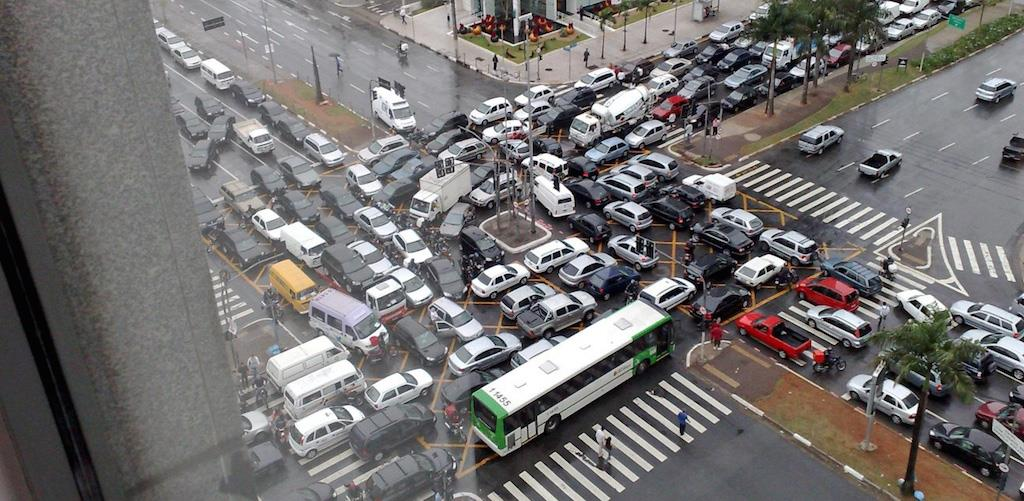
\includegraphics[scale=0.3]{gridlock.png} \\
Imagine a project with hundreds of developers working on it.
\end{frame}

\begin{frame}{Coding as a Team}
One approach might be to have different developers work on separate areas of the code.
\begin{itemize}
\item AKA: Divide and Conquer!
\end{itemize}
In practice, this is pretty common.
\begin{itemize}
\item One developer works on one component (e.g., a library file in C), the next developer works on something else, etc.
\item This is known as code ``ownership''
\item Pros:
\begin{itemize}
\item Developers don't make changes to overlapping areas of code. 
\item Developers build expertise with an area of the code, and can make changes and updates faster.
\end{itemize}
\end{itemize}
\end{frame}

\begin{frame}{Coding as a Team (cont.)}
The problem of course is that:
\begin{enumerate}
\item Coding projects don't always break down that easily
\item We're trusting people to stay in their lane
\item At a certain point the various components need to be integrated.
\end{enumerate}
Thus, the problem of multiple developers working on the same code is unavoidable for large projects.  In addition, there is the \textbf{bus factor} to consider.
\begin{itemize}
\item "The bus factor is a measurement of the risk resulting
from information and capabilities not being shared
among team members, derived from the phrase 'in
case they get hit by a bus'." - Wikipedia
\end{itemize}
\end{frame}

\begin{frame}
\center

\includegraphics[scale=0.8]{modernproblems.jpg}
\end{frame}

\section[Version Control]{Version Control}
\begin{frame}{Enter Version Control}
\textbf{Version Control Systems} manage changes to source code and related file in \textbf{repositories} or colloquially \textbf{repos}.
\begin{itemize}
\item Repositories make it very straightforward to keep your files up-to-date with the latest changes.
\item Whenever changes are committed to the repo, a new version of the files is created.  
\item Developers can access older or alternative versions of the files, so detrimental changes can be reversed!
\item Repos are important in the open source community, as they can be used to manage crowd-sourced coding projects. 
\end{itemize}
\end{frame}

\begin{frame}{Version Control System Usage}
\center
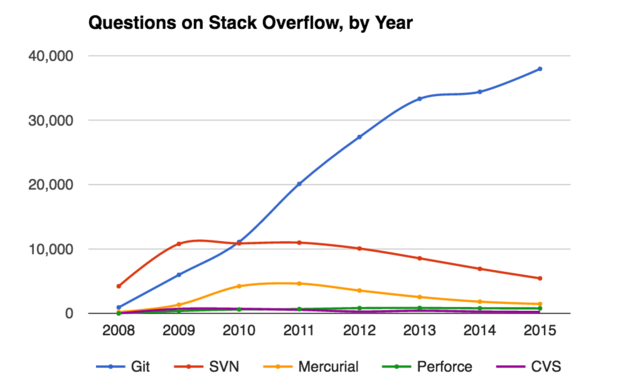
\includegraphics[scale=0.4]{repousage.png}
\end{frame}



\begin{frame}{Git}
\begin{columns}
\begin{column}{0.6\textwidth}
Git was created in 2005 by Linus Torvalds.\\ 
\begin{itemize}
\item That's right folks! The Linux Guy
\item He named it ``git'' because it's British slang for an ``unpleasant person''
\item Apparently, people found him to be a git during coding projects.  
\end{itemize}
\end{column}
\begin{column}{0.38\textwidth}
\fbox{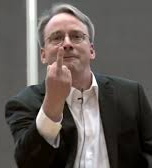
\includegraphics[scale=0.6]{linus.png}}
\end{column}
\end{columns}
\vspace{1em}
Today, the most popular way to obtain a git repository is through the internet service \textbf{github}.  
\begin{itemize}
\item Previously, you had to pay a subscription for private repositories, but since being bought out by Microsoft, private repos are free (with some probable limitations)! 
\end{itemize}
\end{frame}

\begin{frame}{Git (cont.)}
Previous version control systems followed the traditional \textbf{client-server model}. Git uses a \textbf{distributed model}. \\ 
\vspace{1em}
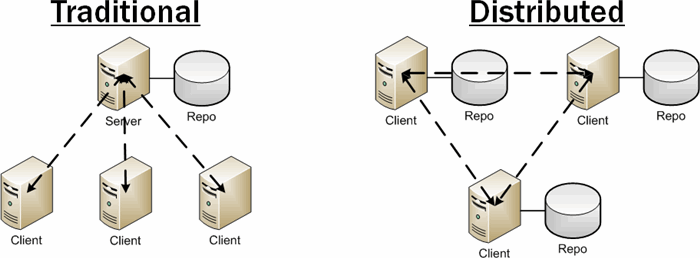
\includegraphics[scale=0.4]{traddist.png}

Though in practical terms, a server is still be necessary to coordinate the distributed clients.  
\end{frame}


\section[Git Basics]{The Basics of Git}
\begin{frame}[fragile=singleslide]{GITting Started!}
Even if github is hosting your repository, you will need the software installed if you don't want to do everything in a web browser.
\begin{itemize}
\item \url{https://git-scm.com/downloads}
\item In general, GUIs are fine to use, but command line is usually faster, and can be integrated into scripts etc.  
\item A professional software developer is expected to understand how to use the command line version.
\end{itemize}
To create a new git repo...
\begin{lstlisting}[style=C, language=bash]
$ git init
Initialized empty Git repository in /[...]/code/.git/
\end{lstlisting}
Files and folders with the \texttt{.} prefix are \emph{hidden files}.  You can view hidden files with \texttt{ls -a}
\end{frame}

\begin{frame}{Git Workflow}
Here are some general procedures for working in a repository (these are applicable to other version control systems!)
\begin{itemize}
\item In a repo, files and directories are either \emph{tracked} or \emph{untracked}.  
\begin{itemize}
\item Only tracked files and folders are a part of the repository.  
\item Files and folders must be \textbf{add}ed to the repository manually.
\end{itemize}
\item As you work on files, periodically \textbf{commit} your changes to the repository.  
\begin{itemize}
\item Think of this as \emph{SUPER} saving your work.
\end{itemize}
\item If you're working on a networked git repo (which is probable), you also have to \textbf{push} your commits to the network.  
\begin{itemize}
\item Doing this every time you commit is a good idea.  
\end{itemize}
\end{itemize}
\end{frame}

\begin{frame}{Basic Git Commands}
We're not talking about server uploads/downloads just yet, just commands operational on local repositories.
\begin{itemize}
\item \texttt{git add <filename>}
\begin{itemize}
\item Tells git to track the specified files and/or folders
\item You can add multiple files as well: 
\begin{itemize}
\item \texttt{git add f1 f2 f3}
\item \texttt{git add *.c}
\end{itemize}
\end{itemize}
\item \texttt{git commit -m "log message"}
\begin{itemize}
\item Commits everything in the working directory and all subdirectories.
\item Commits expect a log message, which can be specified using the \texttt{-m} flag.  
\item If you fail to provide one, git will open up a text editor (like nano) because you probably just forgot, right?
\item Descriptive log messages are important!  Important like good commenting habits!  
\end{itemize}
\end{itemize}
\end{frame}

\begin{frame}{Don't be this guy}
\center
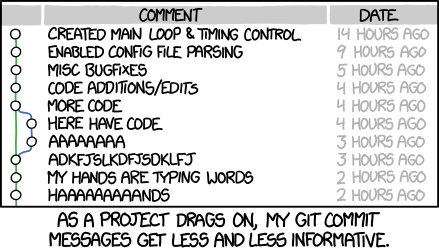
\includegraphics[scale=0.6]{xkcd.png}
\end{frame}

\begin{frame}{Basic Git Commands (cont.)}
\begin{columns}
\begin{column}{0.75\textwidth}
\begin{itemize}
\item \texttt{git status} displays...
\begin{itemize}
\item Which files are and are not being tracked
\item Which files have changed since the last commit
\item The current working branch
\end{itemize}
\end{itemize}
\end{column}
\begin{column}{0.23\textwidth}

\includegraphics[scale=0.15]{octocat.png}
\end{column}
\end{columns}

\begin{itemize}
\item \texttt{git log}
\begin{itemize}
\item Displays the date, time and author of commits on the current branch.
\item Also displays commit ID numbers and lovely log messages! 
\end{itemize}
\item \texttt{git checkout <ID\# or branch name>}
\begin{itemize}
\item Changes your tracked files to the specified commit or branch.
\item You can use this to undo changes and navigate the repository.
\end{itemize}
\end{itemize}
\end{frame}

\begin{frame}{Head Master... Snape!?!}
\center
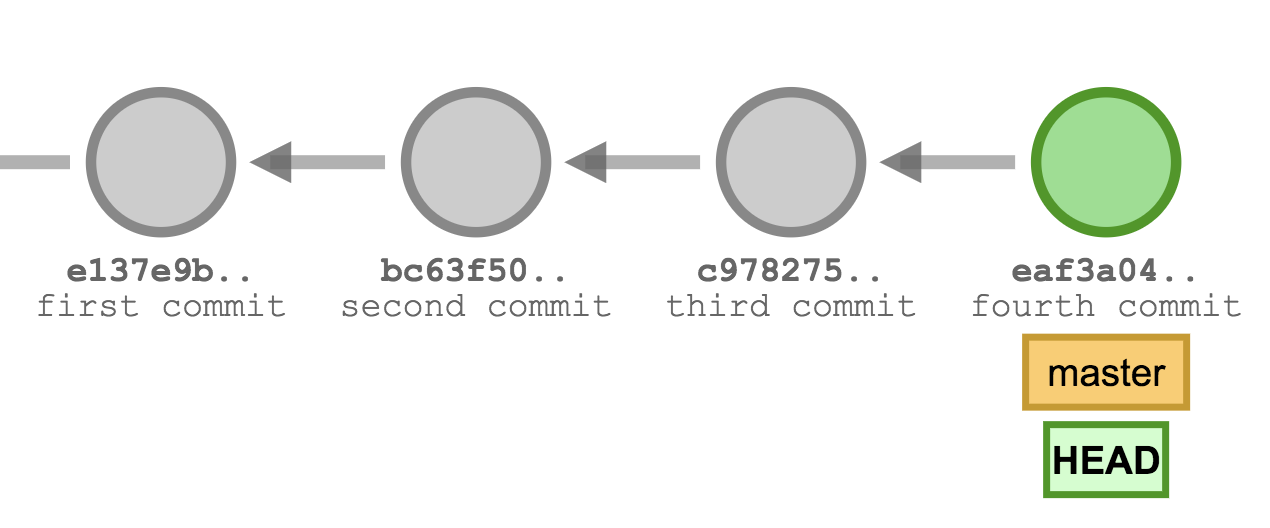
\includegraphics[scale=0.2]{commitchain.png}
\begin{itemize}
\item The \textbf{master} is the default branch created with the repository. 
\item The \textbf{head} of a branch is just the most recent commit.  
\begin{itemize}
\item Checking out a branch automatically takes you to the head of that branch.  
\end{itemize}
\end{itemize}
\end{frame}

\section[Collaboration]{Networking Repositories}
\begin{frame}{So What's the Point of This Again?}
All the foregoing repository management stuff is great and all, but likely overkill for many tasks.
\begin{itemize}
\item It's more applicable than you think, any project of significant size would benefit from this approach.  
\end{itemize}
Where things come alive is the ability to \emph{network} your repositories! 
\begin{columns}
\begin{column}{0.53\textwidth}
\begin{itemize}
\item \texttt{git clone <repo>}
\begin{itemize}
\item Creates a local instance of a remote repository
\end{itemize}
\item \texttt{git push}
\begin{itemize}
\item Transmits commits to the other networked repos
\end{itemize}
\end{itemize}
\end{column}
\begin{column}{0.29\textwidth}
\fbox{
\includegraphics[scale=0.35]{internet.png}} \\ 
\end{column}
\end{columns}
\begin{itemize}
\item \texttt{git pull}
\begin{itemize}
\item Receives commits from the other networked repos and checks out the current head.
\end{itemize}
\end{itemize}
\end{frame}

\begin{frame}{A note on URLs...}
To clone a repo, you first have to know where it is, and what protocol you're using.
\begin{itemize}
\item \texttt{ssh://[user@]host.xz[:port]/path/to/repo.git/}
\item \texttt{git://host.xz[:port]/path/to/repo.git/}
\item \texttt{http[s]://host.xz[:port]/path/to/repo.git/}
\end{itemize}
If your repo is being hosted by GitHub, they have a handy button you can use to get the correct URL:
\center
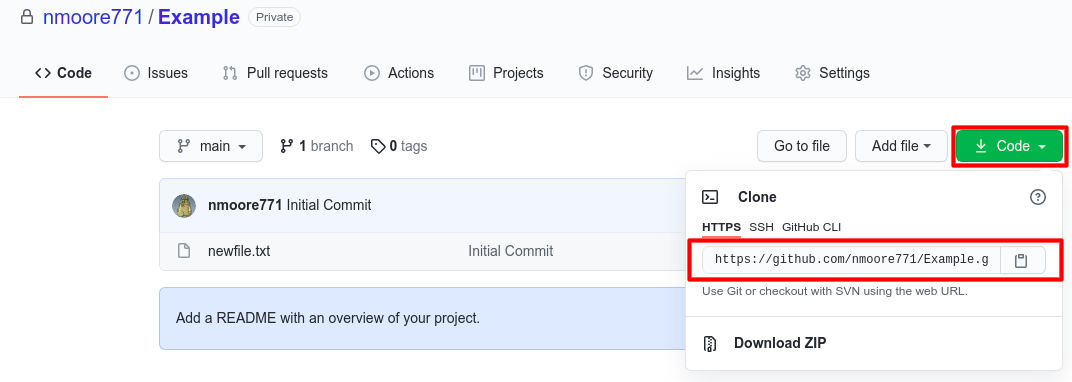
\includegraphics[scale=0.25]{github.png}
\end{frame}

\begin{frame}{Collaborative Workflow}
When working on a project with humans, it is curteous to:
\begin{itemize}
\item Always \texttt{pull} the latest changes \emph{before} you start working.
\item Always \texttt{push} your changes \emph{promptly} when you're done.
\item Document! Your! Changes! Period! Exclamation Mark!
\end{itemize} 
\begin{columns}
\begin{column}{0.48\textwidth}
\fbox{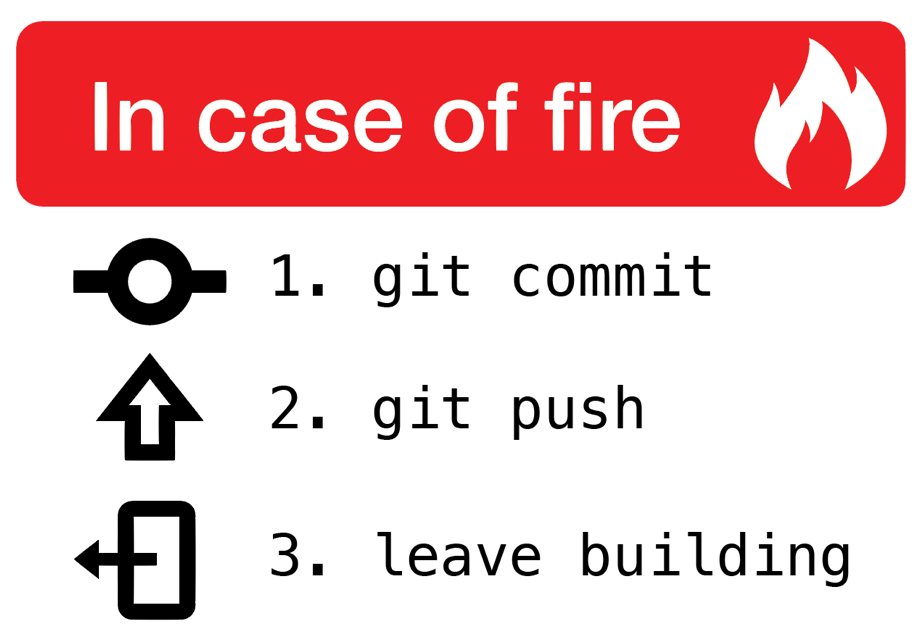
\includegraphics[scale=0.15]{Fire.png}}
\end{column}
\begin{column}{0.48\textwidth}
\begin{itemize}
\item Any major changes (such as new features) should be made in a separate \textbf{branch}, and then \textbf{merged} back into \texttt{master} when the new feature is (mostly) complete.  
\end{itemize}

\end{column}
\end{columns}
\end{frame}

\section[Branches]{Managing Branches}
\begin{frame}{Let me go out on a limb here...}
\textbf{It is your job to keep \texttt{master} stable at all times.} 
\begin{itemize}
\item Adding a feature, or even general development will often break things for a while, and pushing broken code into \texttt{master} is the hieght of bad manners! 
\item Once your branch is finished, you can merge it back into \texttt{master}, often with minimal effort.
\item This way, differen't people's changes remain isolated throughout development. 
\end{itemize}
\center
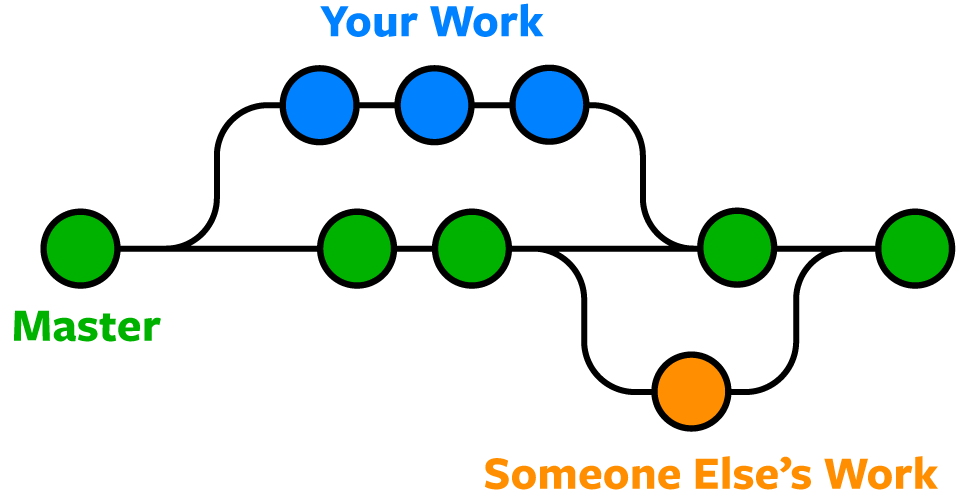
\includegraphics[scale=0.15]{git-branches-merge.png}
\end{frame}

\begin{frame}{Assistant Branch Manager}
Branching is easy!
\begin{itemize}
\item \texttt{git branch <branch name>}
\begin{itemize}
\item Creates a new branch with the given name.
\item You have to switch to the new branch manually if you want to use it.
\end{itemize}
\item \texttt{git switch <branch name>}
\begin{itemize}
\item Switches to the specified branch.  
\item Similar effect to changing your working directory in the file system.  
\end{itemize}
\item \texttt{git log --all} 
\begin{itemize}
\item Displays commits from all branches, not just the active branch.
\end{itemize}
\end{itemize}
\end{frame}

\begin{frame}{Assistant TO the Branch Manager}
\texttt{git log --all --graph} even gives you a visualization: 
\center
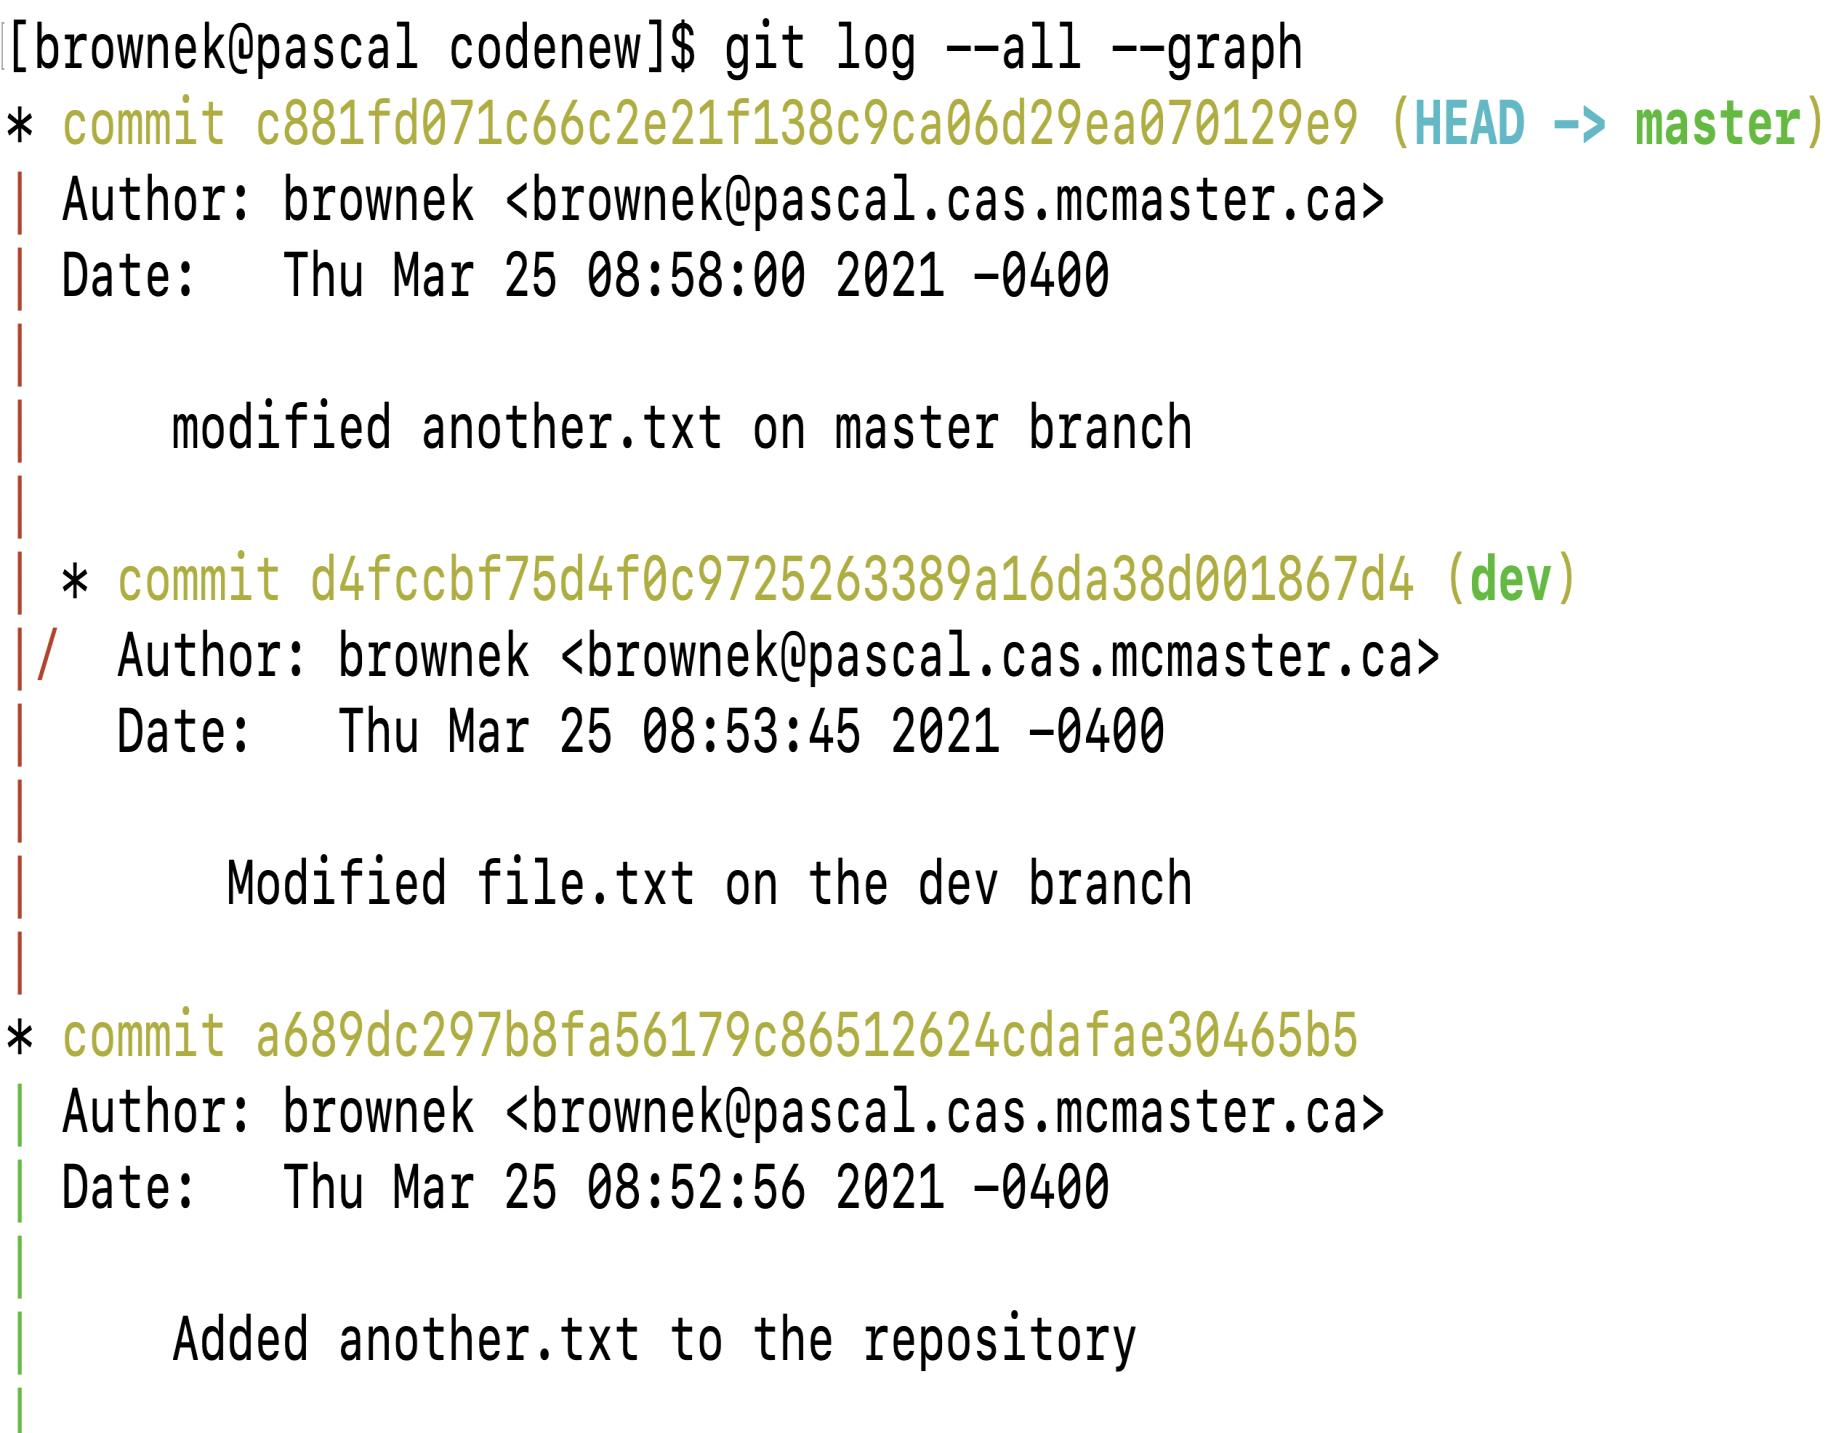
\includegraphics[scale=0.12]{gitlogallgraph.png} 
\end{frame}

\begin{frame}{Why the Fork Not?}
You may notice on GitHub, one of your popularity indicators is the number of \textbf{forks} your repository has.  
\begin{itemize}
\item A \textbf{fork} is a branch operation over an entire repository.
\item Forking is often used to start a new project from an existing one.  
\begin{itemize}
\item LibreOffice was forked from OpenOffice in 2010, because some OpenOffice community members didn't like how Oracle did its licensing for previous open source projects.  
\end{itemize}
\item There's no command for forking with git, but many git GUI tools have a button for it (including GitHub!)
\end{itemize}
\end{frame}

\section[Merging]{Merging Branches}
\begin{frame}{Merge Dragons!}
\texttt{git merge <branch name>} 
\begin{itemize}
\item Merges the specified branch into the currently active branch.
\item You can see which branch you're in by using \texttt{git branch}.
\item Merging requires a commit message, and git will prompt you with one for a text editor if it's missing. 
\end{itemize}
git is pretty clever at merging branches, but there is always a possibility of \textbf{conflicts}.
\begin{itemize}
\item If the changes are in different files in the different branches, merger is trivial! 
\item If the changes are in different parts of the same file, merger is trickier, but will probably work...
\item If the changes are in the same part of the same file, git probably won't be able to figure it out! 
\end{itemize}
\end{frame}

\begin{frame}[fragile=singleslide]{Conflicts in the Workplace}
A \textbf{conflict} happens when a branch merger can't be resolved  automatically.  
\begin{itemize}
\item \textbf{Fixing conflicts is your job as the programmer!}
\item It's tedious and no one likes it.
\end{itemize}
General workflow:
\begin{itemize}
\item When a conflict occurs, git puts something like this in the file with the conflict:
\end{itemize}
\begin{lstlisting}
<<<<<<< HEAD
This text conflicts with the other text.
=======
I am the very model of a modern major general.
>>>>>>> branch_being_merged
\end{lstlisting}
\end{frame}

\begin{frame}{Conflicts of Interest}
\begin{itemize}
\item When this occurs, the easiest way to fix this is to open up the file in your favourite text editor (emacs obviously), and manually make the changes.
\item This requires you to read the conflicting lines and figure out what the solution should be! 
\begin{itemize}
\item If the computer could figure it out, it would have! 
\end{itemize}
\item Once you have resolved the conflicts (or as you are resolving the conflicts), commit and push your changes so that they're fixed for everyone, and not just you! 
\end{itemize}
Fixing conflicts is a \emph{major} pain, and many team workflows have conflict avoidance as a top priority.  
That said, they are inevitable, so you're going to need to figure out how to deal with them!  Rolling back to a previous version, even if it's just a fact-finding mission, can be of critical importance!
\end{frame}

\section[Errata]{Errata}
\begin{frame}{The Last Slide Comic}
\center

\includegraphics[scale=0.35]{meme2.jpg}
\end{frame}

\begin{frame}{Credits}
\center
\vspace{8em}
The contents of these slides were liberally borrowed (with permission) from slides from the Winter 2020 offering of 1XA3 (by Curtis D'Alves), and the Winter 2021 offering of 1XC3 (by Dr. Kevin Browne).  
\end{frame}

\end{document}
